\section{100 - WS 1.1, FA 2.4, FA 2.2, AN 4.3 - Vermögensverteilung - Matura 2. NT - 2017/18}

\begin{langesbeispiel} \item[6] %PUNKTE DES BEISPIELS
Das gesamte Vermögen eines Landes ist häufig sehr ungleich auf die Bevölkerung verteilt. Eine im Jahr 2012 durchgeführte Erhebung der Europäischen Zentralbank (EZB) lieferte Daten für eine Abschätzung, welcher Anteil der österreichischen Bevölkerung über welches Vermögen (in Millionen Euro) verfügt. Die Ergebnisse der darauf basierenden Studie sind in Abbildung 1 dargestellt. Beispielsweise bedeutet der Schwellenwert bei 20\,\%, dass die vermögensschwächsten 20\,\% der österreichischen Bevölkerung ein Vermögen von maximal \EUR{6.086} besitzen.\\
Im Jahr 2012 betrug die Bevölkerungsanzahl von Österreich ca. 8,45\,Millionen Einwohner/innen.

Die sogenannte \textit{Lorenz-Kurve L} (vgl. Abbildung 2) veranschaulicht, welcher relative Anteil der Bevölkerung welchen relativen Anteil des Gesamtvermögens besitzt. So besitzen laut der EZB-Studie die vermögensschwächsten 80\,\% der österreichischen Bevölkerung nur ca. 23\,\% des gesamten Vermögens.

\meinlr[0.1]{Abbildung 1:

\resizebox{0.95\linewidth}{!}{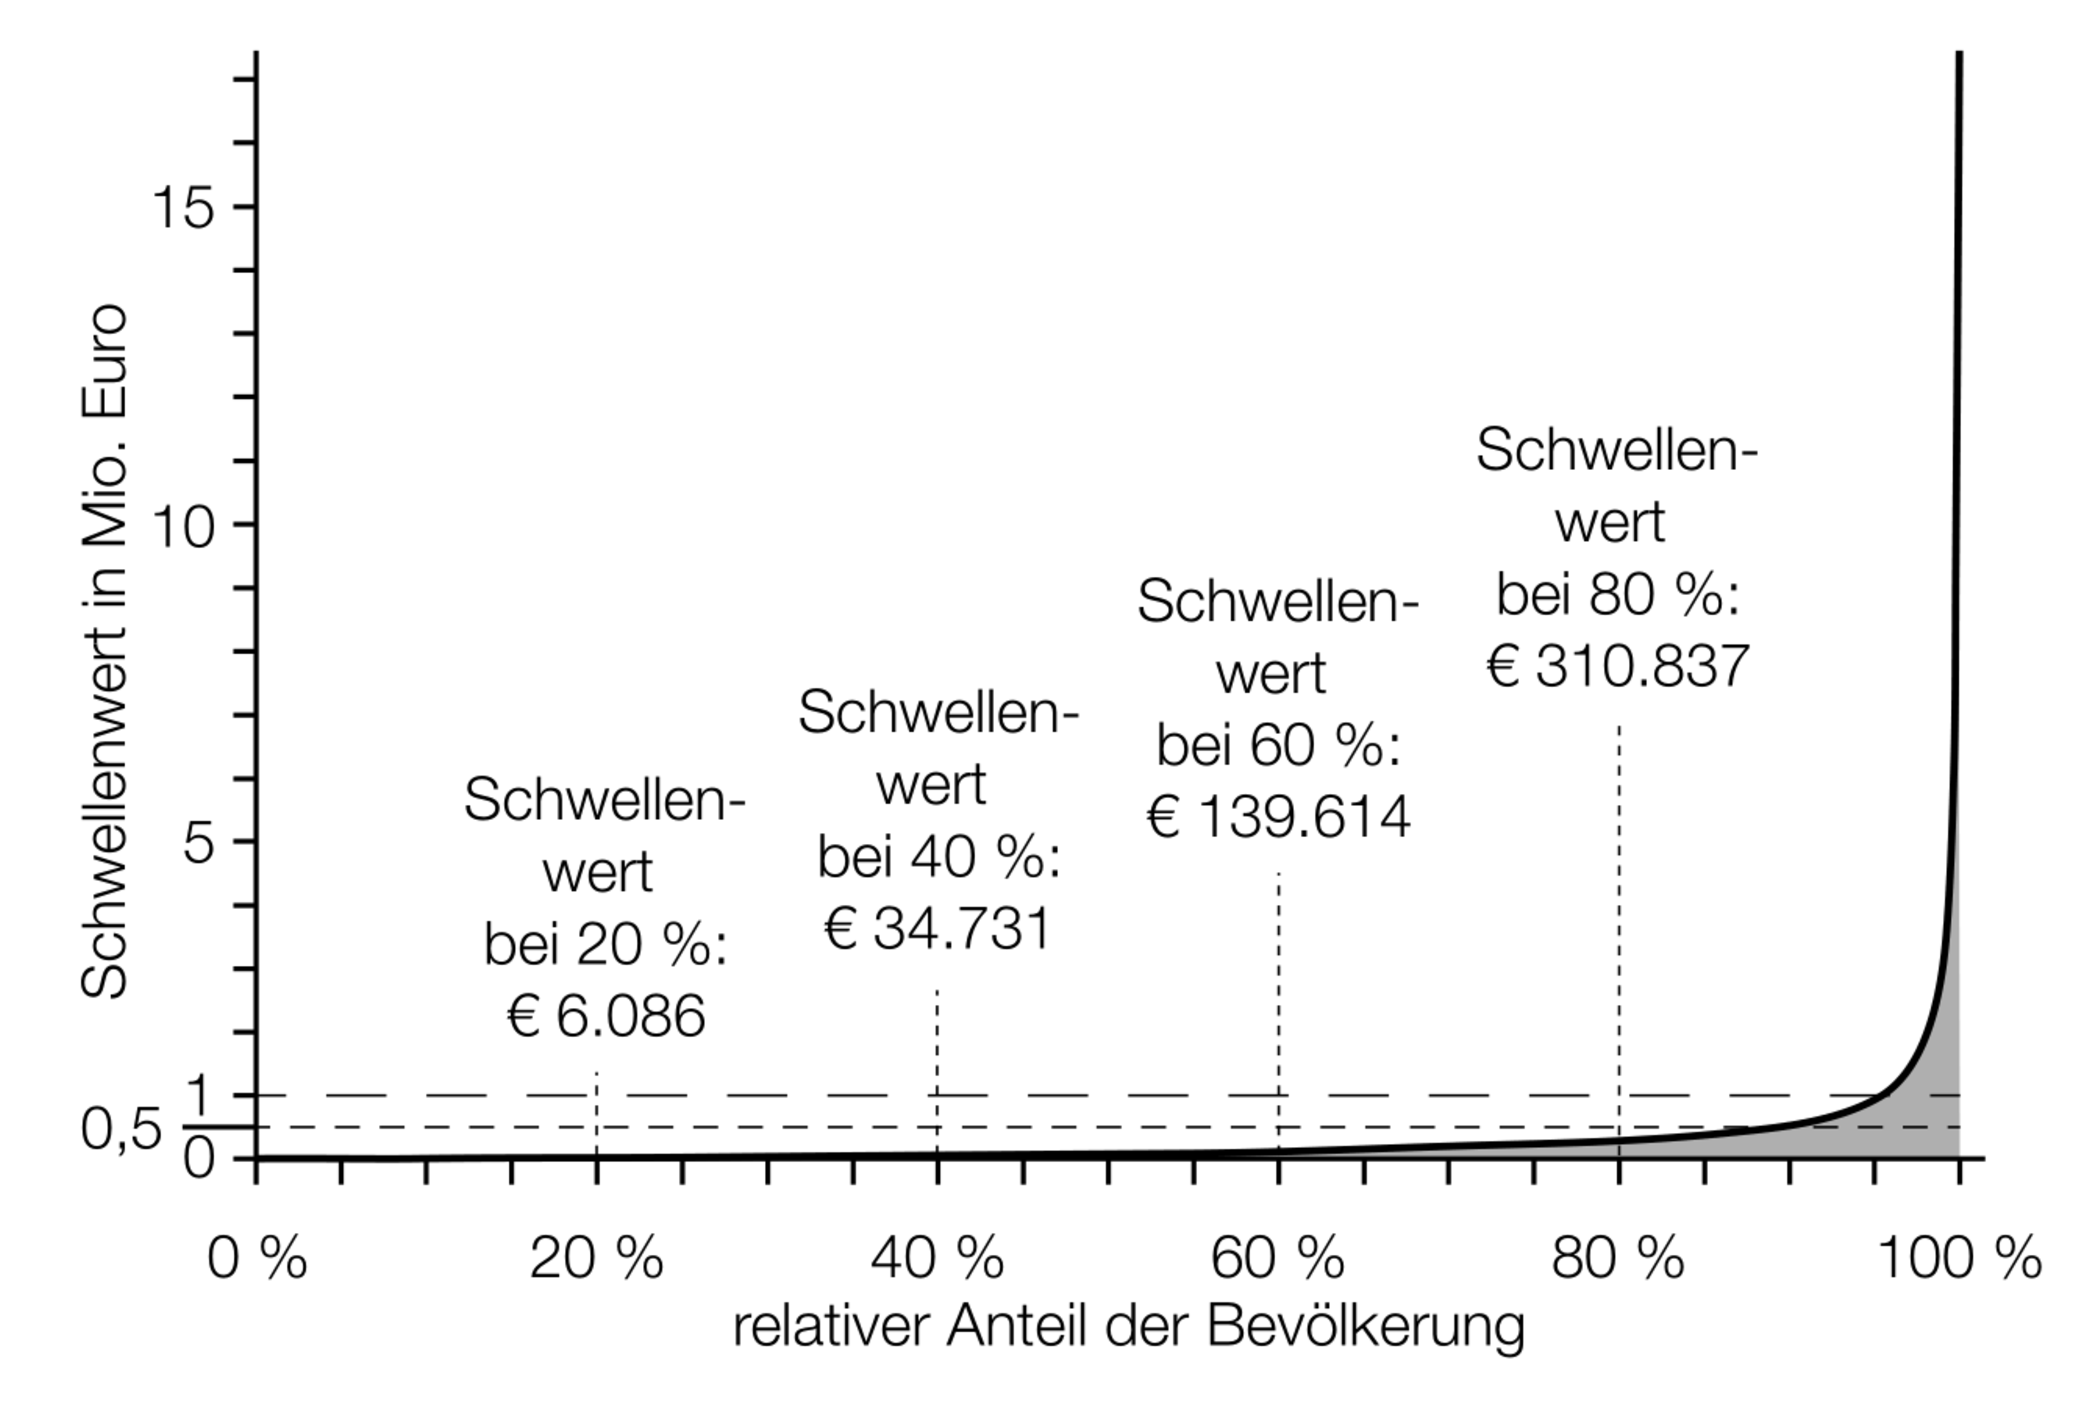
\includegraphics{../_database/Bilder/vermoegen.eps}}}{Abbildung 2:

\resizebox{1.1\linewidth}{!}{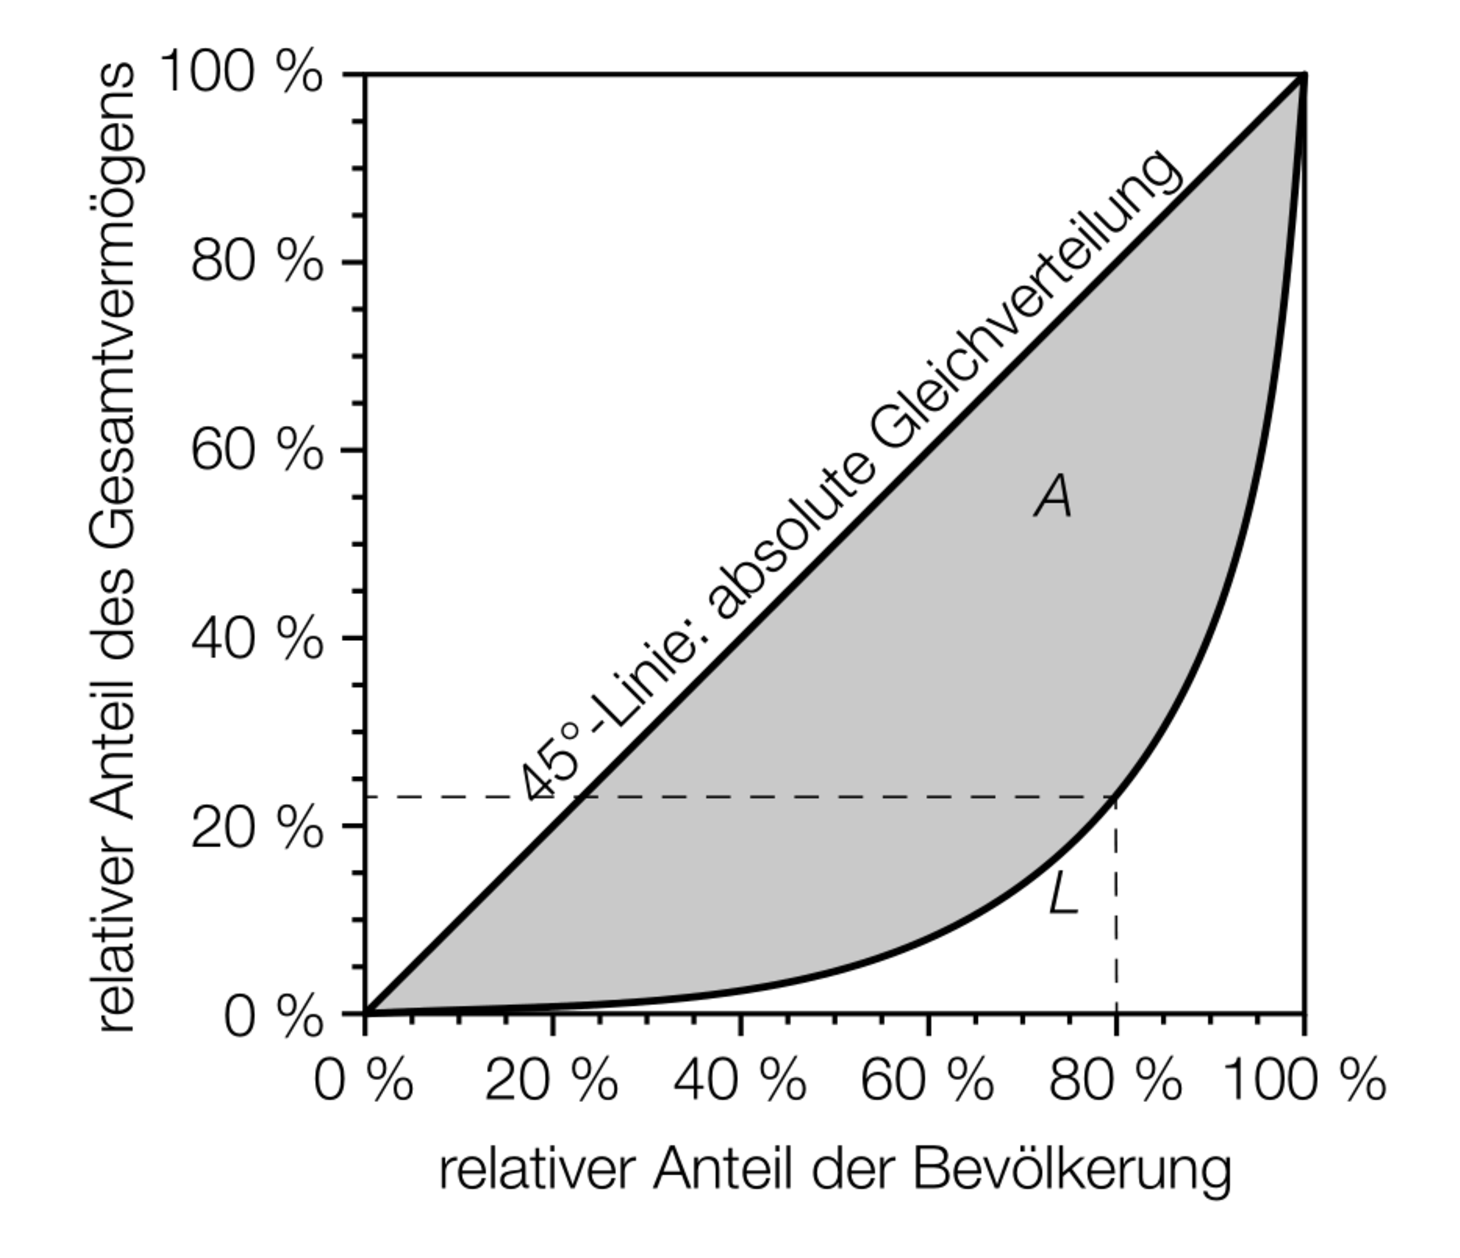
\includegraphics{../_database/Bilder/vermoegen2.eps}}}

\begin{tiny}\begin{singlespace}
Quelle: Eckerstorfer, Paul, Johannes Halak et al.: Vermögen in Österreich. Bericht zum Forschungsprojekt "Reichtum im Wandel".
Linz: Johannes-Kepler-Universität Linz 2013, S. 12-13.
http://media.arbeiterkammer.at/PDF/Vermoegen$\_$in$\_$Oesterreich.pdf [17.10.2014](adaptiert).\end{singlespace}
\end{tiny}

Der Gini-Koeffizient ist ein Maß für die Ungleichverteilung des Vermögens in einem Land. Er entspricht dem Quotienten aus dem Inhalt der markierten Fläche $A$ (zwischen der $45^\circ$-Linie und der Lorenz-Kurve $L$) und dem Flächeninhalt desjenigen Dreiecks, das durch die Eckpunkte $(0\,\%\mid 0\,\%)$, $(100\,\%\mid 0\,\%)$ und $(100\,\%\mid 100\,\%)$ festgelegt ist.\\
Laut EZB-Studie hatte der Gini-Koeffizient für Österreich für das Jahr 2012 den Wert 0,76.

\subsection{Aufgabenstellung:}
\begin{enumerate}
	\item \fbox{A} Ermittle mithilfe von Abbildung 1, wie viele Personen in Österreich im Jahr 2012 ein Vermögen von mindestens einer Million Euro besaßen!
	
	Berechne unter der vereinfachenden Annahme, dass die Schwellenwerte im Intervall $[20\,\%; 40\,\%]$ annähernd linear zunehmen, einen Näherungswert des Schwellenwerts bei $25\,\%$!
	
	\item Ermittle, welchen relativen Anteil am Gesamtvermögen die vermögensstärksten 10\,\% der österreichischen Bevölkerung besitzen!
	
	Laut einer Studie der Universität Linz aus dem Jahr 2013 besitzen die vermögensstärksten 10\,\% der österreichischen Bevölkerung einen deutlich relativen Anteil am Gesamtvermögen, als es in der EZB-Studie behauptet wurde.
	
	Unter Berücksichtigung der Studie der Universität Linz erhält man eine andere Lorenz-Kurve $L^*$ als die abgebildete Lorenz-Kurve $L$. Skizziere in der nachstehenden Abbildung einen möglichen Verlauf einer solchen Lorenz-Kurve $L^*$!
	
	\begin{center}
	\resizebox{0.7\linewidth}{!}{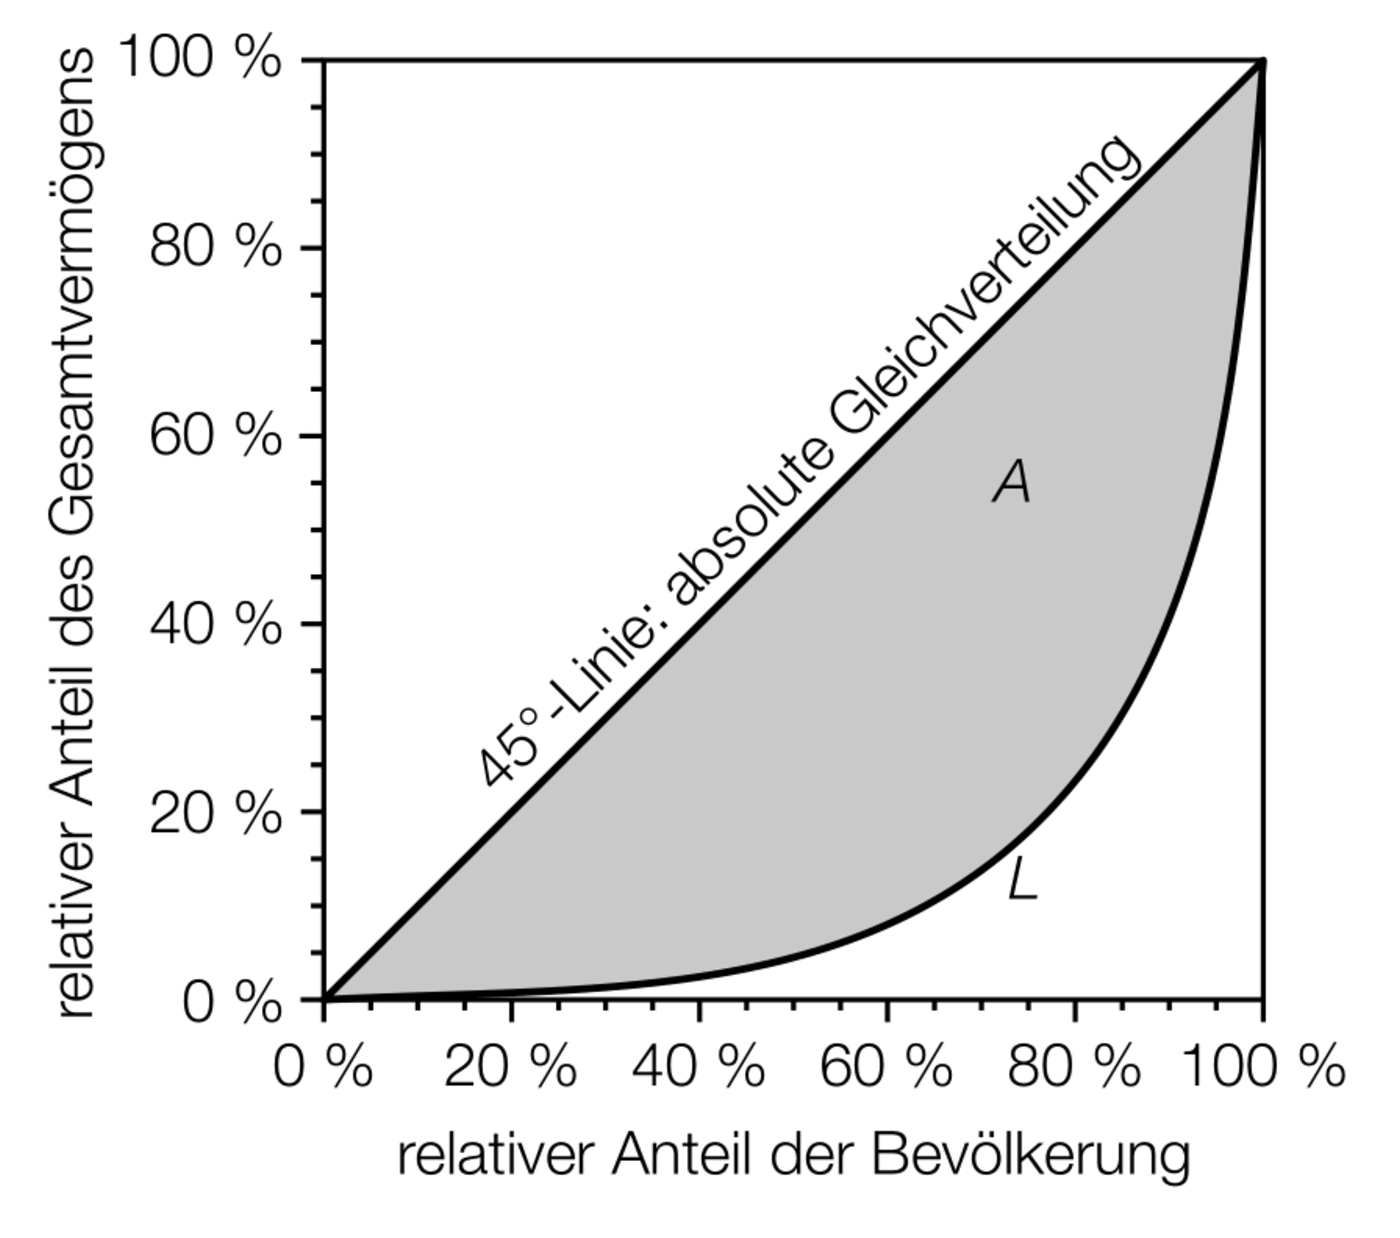
\includegraphics{../_database/Bilder/vermoegen3.eps}}
	\end{center}
	
	\item Die Lorenz-Kurve wird im Intervall $[0;1]$ durch eine relle Funktion in Abhängigkeit von $x$ modelliert, wobei $x$ den relativen Anteil der Bevölkerung angibt.
	
	Berechne den Gini-Koeffizienten für ein Land $S$ dessen Lorenz-Kurve für das Jahr 2012 durch die Funktion $L_1$ mit $L_1(x)=0,9\cdot x^5+0,08\cdot x^2+0,02\cdot x$ im Intervall $[0;1]$ beschrieben werden kann.
	
	Vergleiche dein Ergebnis mit dem Gini-Koeffizienten für Österreich für das Jahr 2012 und gib an, ob das Gesamtvolumen in diesem Jahr in Österreich oder im Land $S$ gleichgemäßiger auf die Bevölkerung verteilt war!
\end{enumerate}

\antwort{
\begin{enumerate}
\item \subsection{Lösungserwartung:}

Im Jahr 2012 hatten in Österreich ca. 422\,500 Personen (laut Abbildung 1: ca. $5\,\%$ der Bevölkerung) ein Vermögen von mindestens eine Million Euro.

Mögliche Vorgehensweise:\\
$6086+\frac{34\,731-6086}{4}=13\,247,25$\\
Der Näherungswert für den Schwellenwert bei $25\,\%$ liegt bei ca. \EUR{13.247}.

\subsection{Lösungsschlüssel:}
\begin{itemize}
\item Ein Ausgleichspunkt für die richtige Lösung, wobei auch die Angabe des richtigen relativen Anteils als richtig zu werten ist.\\
Toleranzintervalle: $[338\,000; 507\,000]$ bzw. $[4\,\%; 6\,\%]$.
\item Ein Punkt für die richtige Lösung, wobei die Einheit "\euro "nicht angeführt sein muss.\\
Toleranzintervall: $[$\EUR{13.200}; \EUR{13.325}$]$
\end{itemize}

\item \subsection{Lösungserwartung:}

Die vermögensstärksten 10\,\% der österreichischen Bevölkerung besitzen ca. 60\,\% des Vermögens.

Möglicher Verlauf von $L^*$:
\begin{center}
\resizebox{0.5\linewidth}{!}{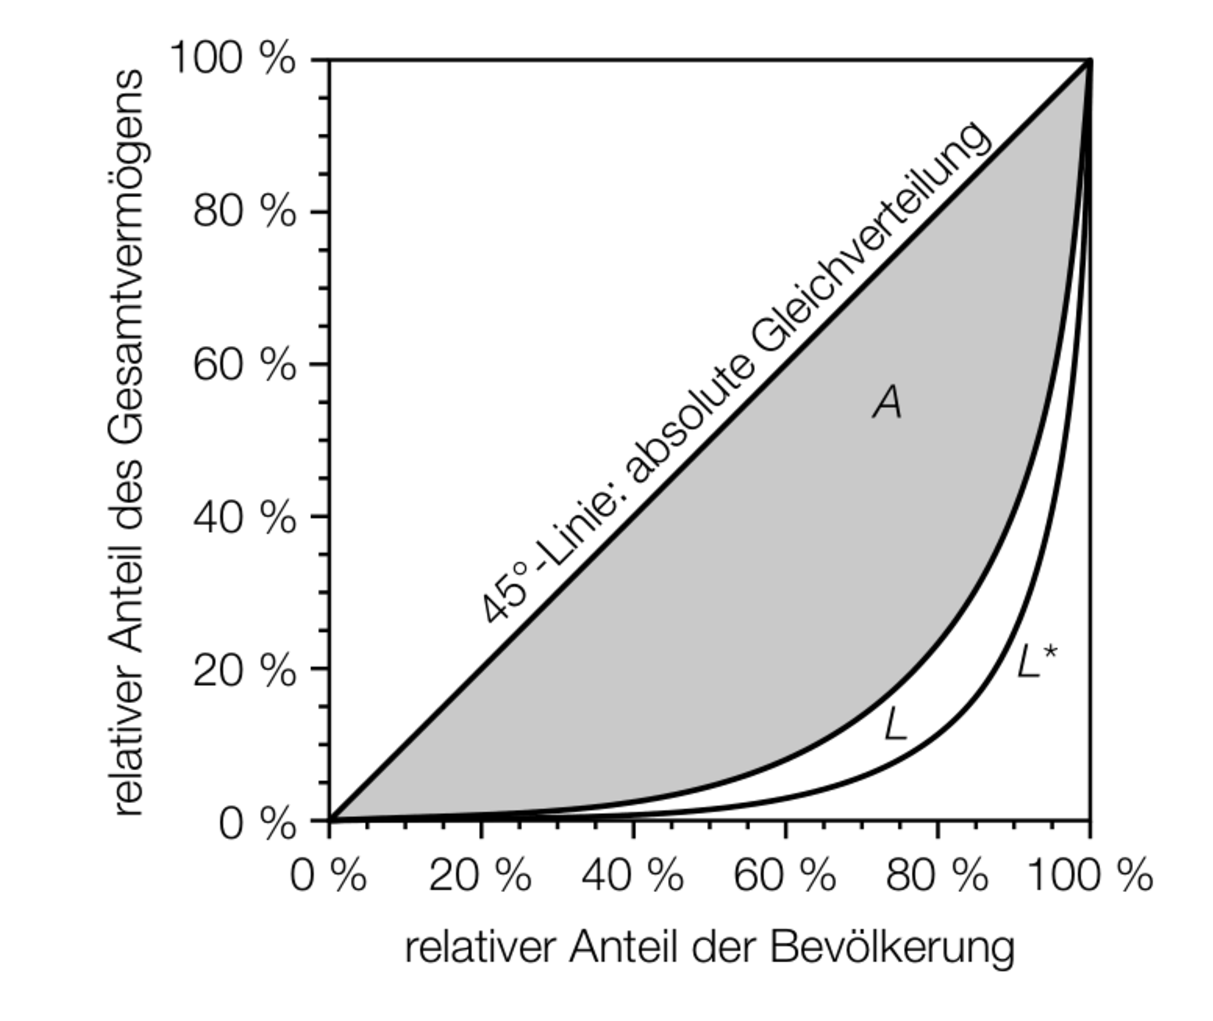
\includegraphics{../_database/Bilder/vermoegen4.eps}}
\end{center}

\subsection{Lösungsschlüssel:}
\begin{itemize}
\item Ein Punkt für die richtige Lösung.\\
Toleranzintervall: $[58\,\%; 62\,\%]$
\item Ein Punkt für einen richtig eingezeichneten Verlauf einer möglichen Lorenz-Lurve $L^*$, wobei der Funktionswert an der Stelle 90\,\% kleiner als 42\,\% sein muss und die Funktion monoton steigend sein muss.
\end{itemize}

\item \subsection{Lösungserwartung:}

Mögliche Vorgehensweise:\\
$0,5-\displaystyle\int^1_0 L_1(x)\,\text{d}x=0,31\dot{3}$

$\dfrac{0,31\dot{3}}{0,5}\approx 0,63$

Der Gini-Koeffizient für das Jahr 2012 hatte für das Land $S$ etwa den Wert 0,63.

Der Gini-Koeffizient für das Jahr 2012 war für das Land $S$ niedriger als jener für Österreich. Das bedeutet, dass in diesem Jahr das Gesamtvermögen im Land $S$ gleichmäßiger auf die Bevölkerung verteilt war als in Österreich.

\subsection{Lösungsschlüssel:}
\begin{itemize}
\item Ein Punkt für die richtige Lösung.\\
Toleranzintervall: $[0,62; 0,63]$\\
Die Aufgabe ist auch dann als richtig gelöst zu werten, wenn bei korrektem Ansatz das Ergebnis aufgrund eines Rechenfehlers nicht richtig ist.
\item Ein Punkt für einen korrekten Vergleich und eine (sinngemäß) richtige Deutung.
\end{itemize}

\end{enumerate}}
\end{langesbeispiel}